% ==================================================
% CHAPTER 2: Characterization of sTGCs using cosmic rays %
% ==================================================

% Note: in intro you'll need to introduce pads, strips and wires == electrodes.

\chapter{Characterization of sTGCs using cosmic rays}
\label{chap:cosmics}
% Edit count: Lia - 0, Brigitte - 0

In Canada, the cathode boards were prepared at TRIUMF in Vancouver; the quadruplets were constructed at Carleton University in Ottawa; and the completed quadruplets were tested and characterized with cosmic muons at McGill University in Montreal~--- before being sent to CERN. In this chapter pertinent details of cosmic muon testing at McGill are presented. 

% --------------------------------------------------
\section{Collecting cosmic muon data}
% --------------------------------------------------

Cosmic muon characterization was done with a typical hodoscope.  The quadruplet was placed in the test bench (of which a complete description can be found in~\cite{lefebvre_thesis}). Above and below it was a layer of scintillator-PMT arrays, labelled in figure~\ref{fig:hodoscope}. If any one scintillator from each array fired in coincidence, it indicated the passage of a cosmic muon to be recorded by the quadruplet. The trigger was passed \iffalse through a KC705\footnote{Xilinx, Xilinx Kintex-7 FPGA KC705 Evaluation Kit, EK-K7-KC705-G, 2018} which sent it \fi to the front end boards (FEBs) attached to the adaptor boards of each layer of the quadruplet, which readout the electrodes.

\begin{figure}
    \centering
    \includegraphics[width = 0.9\textwidth]{figures/figure_test_bench.png}
    \caption{Cosmic muon hodoscope at McGill University with sTGC quadruplet in position.}
    \label{fig:hodoscope}
\end{figure}

% It would be great to have a scope trace here, preferably of a strip. Oops.
Each sTGC electrode was connected to a channel on an ASIC\footnote{the VMM3~\cite{iakovidis_vmm3_2017} \textcolor{red}{check this in lab}} on the FEB, which was set to measure and record the channel's maximum output (called peak detector output, or PDO) if the channel was above threshold. Thresholds were measured~\cite{chen_calibration_2019} and adjusted manually in the configuration/readout software~\cite{siyuan_sun_stgc_readout_sw}. For each trigger, the PDO of all channels above threshold were recorded and stored in a binary file, which could be decoded into a usable ROOT tree~\cite{ROOT} by \package{tgc\_analysis/vmm3Decoder}~\cite{lefebvre_tgc_analysis}. A event recorded in the tree corresponded to one trigger from the scintillator-PMT arrays. 

Operating the chambers also required gas and high voltage. A pentane-CO$_{2}$ mixture was created and delivered to each sTGC with a gas system controlled by a slow control program~--- both the gas system and control program were designed and made at McGill~\cite{keyes_development_2017}. High voltage was provided by CAEN boards. Cosmic muon data was collected at 2.9~kV and 3.1~kV. Although the chambers will be operated at 2.8~kV in ATLAS, an earlier version of the FEBs was used at McGill that had a worse signal-to-noise ratio. Separately pad signals sufficiently from noise required operating at 3.1~kV to increase the chambers' gain while 2.9~kV, closer to the nominal voltage, was sufficient for strip and wire signals. Collecting 1 million triggers at each voltage provided enough statistics to calculate characterization metrics, which meant collecting data for just over two hours per quadruplet per voltage.

% --------------------------------------------------
\section{Rebuilding cosmic muon tracks for characterization}
% --------------------------------------------------

The package \package{tgc\_analysis/CosmicsAnalysis}~\cite{lefebvre_tgc_analysis} was used to analyze cosmic muon data and calculate high-level characterization metrics. Many of the characterization methods were based on rebuilding muon tracks. For events passing quality cuts, the x and y coordinates of the ionization avalanche on each layer were extracted from the signal on the wires and strips respectively for each event, as is sketched in figure~\ref{fig:mwpc_coords}.

The x-coordinate was taken as the center of the wire group with the maximum PDO, since the wire groups' pitch (\SI{36}{\milli\meter}) was larger than the typical charge spreading. Assuming that the true x-position of the hit was uniformly distributed over the width of the wire group, the uncertainty in the x-position was given by $\frac{36 mm}{\sqrt{12}} = 10 mm$~\cite{Sauli:117989}.

The y-coordinate was taken as the Gaussian mean of the PDO distribution across groups of contiguous strips. The process of grouping contiguous strips with signal above threshold\footnote{Note that during cosmic ray testing, the hardware was configured to also record the PDO of strips adjacent to a strip above threshold.} was called clustering, and the resulting group was called a cluster. Figure~\ref{fig:mwpc_coords} helps to sketch out the clustering process and a sample cluster is shown in figure~\ref{fig:sample_cluster}. 

\begin{figure}
    \centering
    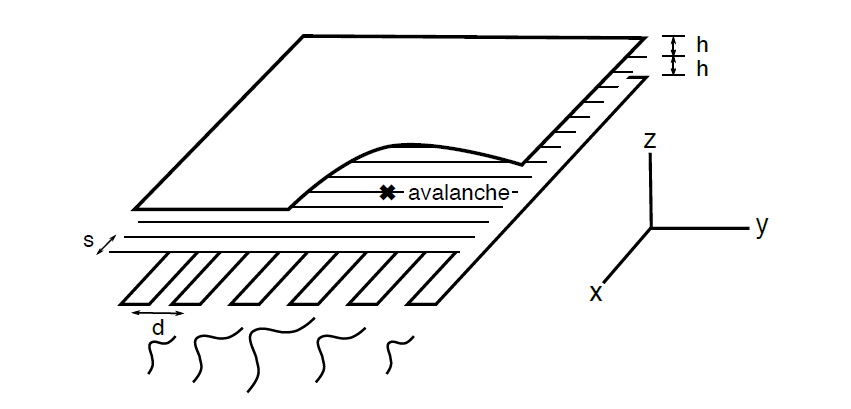
\includegraphics[width = 0.7\textwidth]{figures/mwpc_lefebvre_thesis_gatti.png}
    \caption{A sketch of an sTGC-like detector. The position of the avalanche could be extracted from the wires and strips that picked up the avalanche signal. The signals on individual strips are sketched. Clustering was the processs of fitting a Gaussian to the peak value of the individual contiguous strips, as is done in figure~\ref{fig:sample_cluster}. In this work, the x(y)-coordinate will always refer to the coordinate perpendicular to the wires (strips)~\cite{lefebvre_thesis, gatti_optimum_1979}.}
    \label{fig:mwpc_coords}
%\end{figure}
    \vspace*{\floatsep}
%\begin{figure}
    \centering
    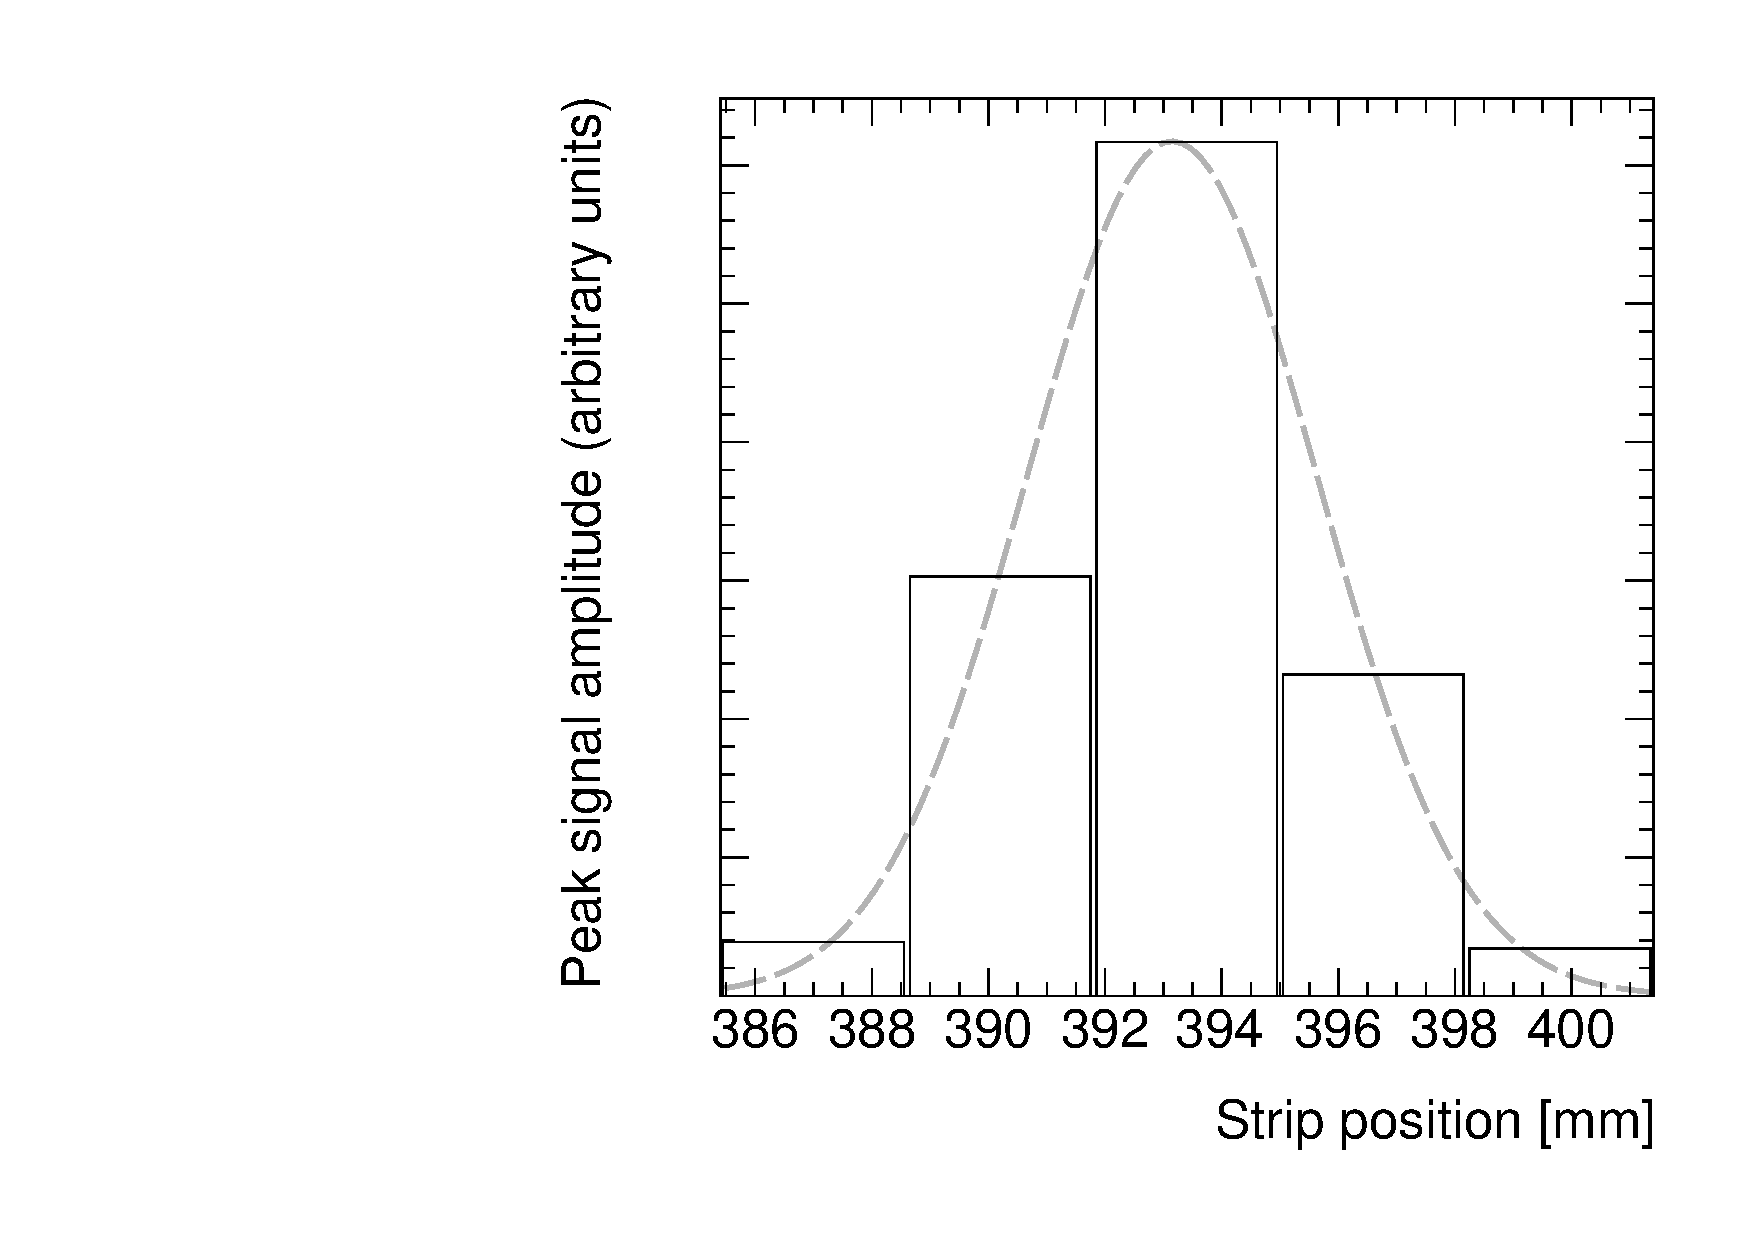
\includegraphics[width = 0.5\textwidth]{figures/sample_cluster_QL2C04_event5_layer2.pdf}
    \caption{A sample cluster resulting from the current picked up on a group of strips (presumably) after the passing of a muon. The grey line is a Gaussian fit.}
    \label{fig:sample_cluster}
\end{figure}

The uncertainty in the cluster mean could be taken as the fitted mean's statistical uncertainty; however, after comparing the difference in cluster means for different fitting algorithms in appendix~\ref{sec:appendix_clustering_cluster_fit}, \SI{60}{\micro\meter} of uncertainty was assigned to the cluster means for the work in this thesis.

The coordinates of the avalanches' on all layers were used to reconstruct tracks in x and y respectively. Most tracks passing quality cuts were probably cosmic muons, but of course $\delta$-rays and noise contributed. The tracks were then used to calculate characterization metrics like electrode efficiency and spatial resolution, the details of which are discussed in~\cite{lefebvre_thesis}.

%TODO : Include hit and track map? - yes if Brigitte says you need a num_entries plot in chapter 3. You didn't include it because you never mention wire supports in TH2 analysis. But if you want to add num entries for clarity, include cluster map here. Cluster map > raw hits because less cuts and gets across the idea that x is just hit or no hit while y comes from clustering. 